\section{LO4: Grammar of Graphics Tools}

The Grammar of Graphics is a comprehensive framework for creating statistical graphics that maps data to visual representations. It decomposes the process of visualization into a series of explicit steps, providing clarity and flexibility in the design of visualizations.

The idea of the Grammar of Graphics was first introduced by Leland Wilkinson in his 1999 book of the same name. It has since been implemented in various statistical graphics packages, including ggplot2 for R and Altair for Python \cite{wilkinsonGrammarGraphics2005, wickhamLayeredGrammarGraphics2010,valero-moraGgplot2ElegantGraphics2010}. The Grammar of Graphics has significantly contributed to advances in data visualization, especially in visualizing multi-dimensional data and large datasets \cite{meyerVisualizationData2000}.

\subsection{Data}
The starting point for any graphic is the dataset. In the Grammar of Graphics, data is considered as a collection of variables. Each variable can be either continuous (e.g., GDP per capita, life expectancy) or categorical (e.g., continent, country). The Gapminder dataset includes both types, offering a rich source for visualization.

\subsection{Aesthetics}
Aesthetics, or aesthetic attributes, are the visual properties of the graphic that can be perceived. These include position (x and y axes), size, shape, color, and transparency. In the context of the Gapminder dataset, we can map the GDP per capita to the x-axis, life expectancy to the y-axis, population size to the point size, and continent to the point color in a scatter plot.

\subsection{Geometric Objects}
Geometric objects or "geoms" are the visual elements that represent data points in a graphic. The Gapminder dataset allows us to use various geoms such as points (for scatter plots), lines (for time series), and bars (for bar charts). For instance, a line geom could be used to represent the trend in life expectancy over time for each country.
An example of a point geom is shown in Figure \ref{fig:lo2_scatter_plot} where the life expectancy and GDP per capita are plotted for each country in the year 2007.

\subsection{Statistical Transformations}
These are the algorithms applied to the data to produce summarized or processed values, like means or medians. In the Gapminder visualization, we could apply a statistical transformation to calculate the average life expectancy and GDP per capita for each continent over time.

\subsection{Scales}
Scales map the values in the data space to the aesthetic dimensions. They can be linear, logarithmic, or categorical. For instance, we might use a logarithmic scale for the GDP per capita in the Gapminder data to account for its wide range and skewness.

\subsection{Coordinate Systems}
The coordinate system, such as Cartesian or polar, determines the framework in which the data is plotted. Most Gapminder visualizations will use a Cartesian coordinate system, which is suitable for most statistical graphics.

\subsection{Facets}
Faceting is a technique to create multiple plots based on a subset of the data, which is particularly useful for comparing different groups. With the Gapminder dataset, we could create facets for each continent to compare the metrics across different regions.
An example of a facetted plot for the data set is shown in Figure \ref{fig:lo4_facet} where the life expectancy over time is plotted for each continent making it and perfect example of a facetted plot.

\begin{figure}[h]
    \centering
    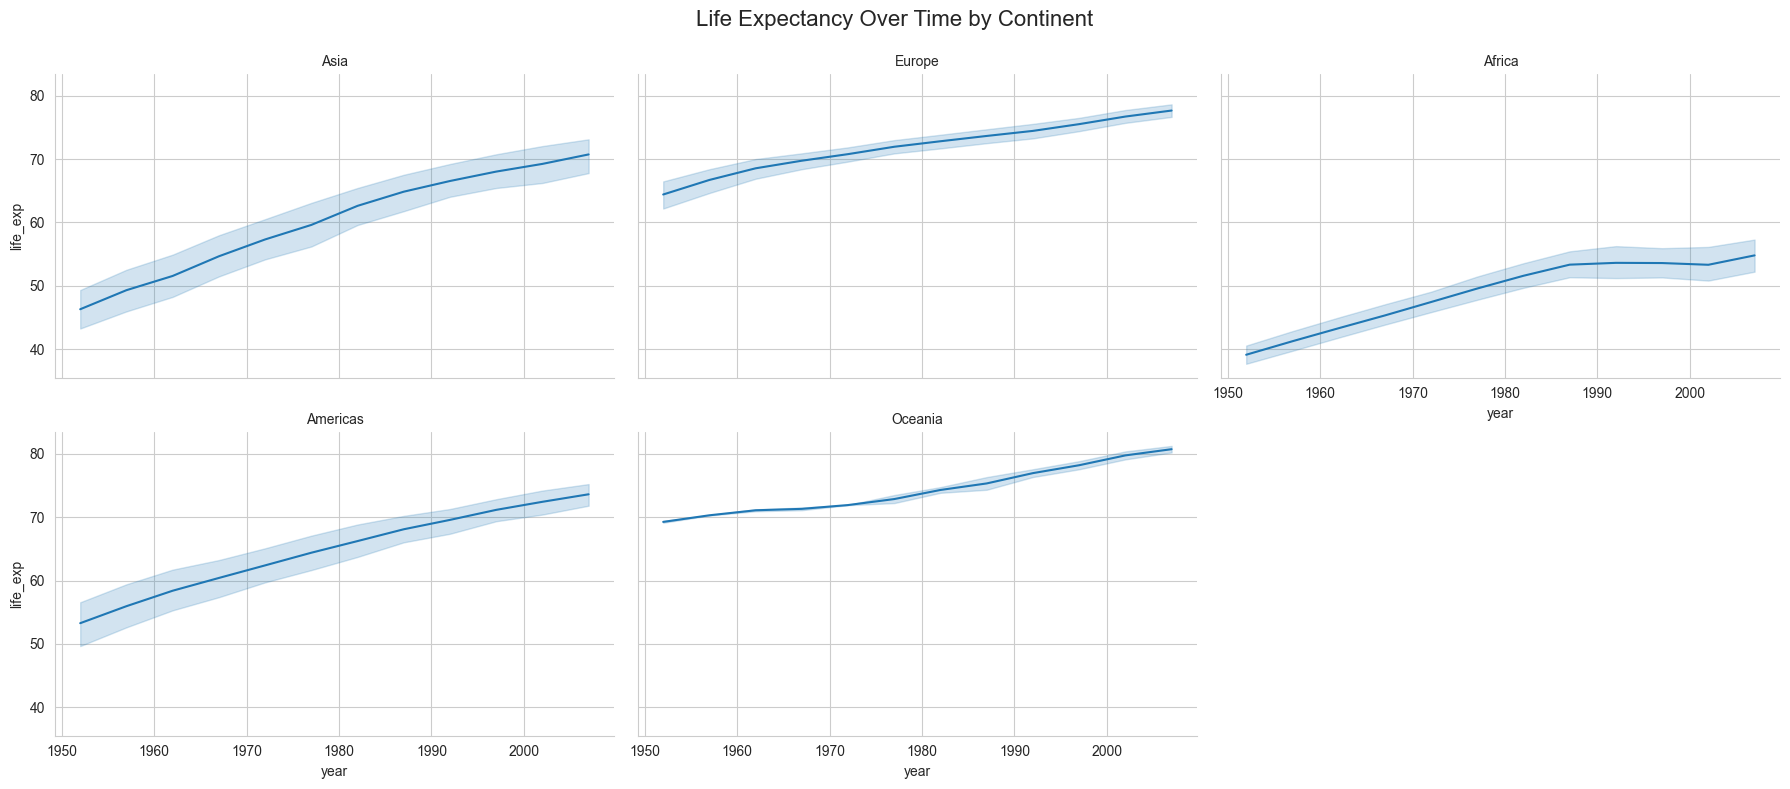
\includegraphics[width=0.8\textwidth]{images/plots/lo4_life_expectancy_over_time_by_continent.png}
    \caption{Change in Life Expectancy Over Time by Continent in a Facetted Plot}
    \label{fig:lo4_facet}
\end{figure}

\subsection{Conclusion}
By understanding and applying the Grammar of Graphics, we can create meaningful and insightful visualizations of the Gapminder dataset. Each component plays a specific role in ensuring that the final graphic is not only visually appealing but also analytically precise.